\documentclass[a4paper,11pt]{article}

\usepackage{jcappub}
\usepackage{txfonts}
\usepackage{threeparttable}
\usepackage{aas_macros}
\usepackage{graphicx}
\usepackage{subfigure}


\title{Precision cosmology with time delay lenses: high resolution imaging requirements}
%\title{Cosmology with time delay lenses. High resolution imaging requirements}
\author[1]{Xiao-Lei Meng,}
\author[1,2]{Tommaso Treu,}
\author[1,2]{Adriano Agnello,}
\author[3]{Matthew W.~Auger,}
\author[1,2]{Kai Liao,}
\author[4]{Philip J. Marshall}

\affiliation[1]{Department of Physics, University of California, Santa Barbara, CA 93106, USA}
\affiliation[2]{Physics and Astronomy Building, 430 Portola Plaza, Box 951547, Los Angeles, CA 90095-1547, USA}
\affiliation[3]{Institute of Astronomy, UK}
\affiliation[4]{Kavli Institute for Particle Astrophysics and Cosmology, Stanford University, 452 Lomita Mall, Stanford, CA 94305, USA}

\emailAdd{xlmeng919@gmail.com}

\date{Accepted . Received }

\abstract{
Gravitational time delays are a powerful probe of cosmology, provided
that the gravitational potential of the main deflector can be modeled
with sufficient precision. Recent work has shown that this can be
achieved by detailed modeling of the host galaxies of lensed
quasars. The distortion of the images as measured over large number of
pixels provides tight constraints on the difference between the
gravitational potential between the two quasars, and thus on cosmology
in combination with the measured time delay. We carry out a systematic
exploration of the high resolution imaging required to eploit the
thousands of lensed quasars that will be discovered by current and
upcoming surveys with the next decade. Specifically we simulate
realistic lens systems as imaged by the Hubble Space Telescope (HST), James Webb Space Telescope (JWST), ground
based adaptive optics images taken with Keck or the Thirty Meter
Telescope (TMT). We compare the performance of these pointed observations
with that of images taken by the Euclid-VIS, Wide-Field Infrared Survey Telescope (WFIRST) and  Large Synoptic Survey Telescope (LSST) surveys. Using
as our metric the precision with which the slope of the mass density
profile for the main deflector can be measured we find that...
}

\keywords{}

\begin{document}
\maketitle
\flushbottom


\section{Introduction}
This paper is organized as follows. We first introduce our lens sample in Section 2. Next, we briefly summarize a variety of telescopes properties used in this work and show how simulate realistic lens systems as imaged by these telescopes in Section 3, and present the results from simulation in Section 4. Finally, we discuss and summarize our work in Section 5. Throughout this paper, all magnitudes are given in AB scale. We assume spatially flat $\Lambda$CDM model with $\Omega_{\rm{m}} = 0.3$, $\Omega_{\Lambda} = 0.7$, and the Hubble constant $H_{0} = 70~\rm km~s^{-1}~Mpc^{-1}$ when calculating distances.


\section{The Lens Sample}
The gravitational lens systems presented in this work were all selected intensively. Here we introduce our sample, a set of 4 lens systems, including 2 realistic systems from observational data and 2 assumed systems based on realistic ones.

\subsection{Selected Realistic Lens Systems}
For wider analysis we plan to We choose a lens from the Sloan Lens ACS Survey (SLACS; Bolton et al. 2008 \cite{2008ApJ...682..964B}; Auger et al. 2009 \cite{2009ApJ...705.1099A})

\section{Simulations}


\subsection{Hubble Space Telescope}
\subsubsection{ACS}
\subsubsection{WFC3}
\subsection{JWST}
\subsection{Keck 10m Telescope}
\subsubsection{LGSAO-NIRC2}
\subsubsection{NGAO}
\subsection{Thirty Meter Telescope}
\subsubsection{IRIS}
\subsection{Euclid}
\subsection{WFIRST}
\subsection{LSST}

\section{Results}

\section{Summary}

\section*{Acknowledgments}







\bibliographystyle{JHEP}
\bibliography{references}

\clearpage
% ===============================================
\begin{table*}\footnotesize
\begin{center}
\caption{Telescope Properties}
\begin{tabular}{lcccccccccccccc|}
\hline \hline
Telescope Name & Filter & Zero Point & Readout & Background & Pixel Scale \\
& & & (-e/pixel/s) & (-e/pixel/s) & (arcsec) \\
\hline
HST    &   F814W   &   25.94    &   4.20      &    0.11     &     0.050    \\
  JWST   &   F200W   &    27.85   &    9.00     &     0.20    &      0.032  \\
  Keck   &   NIRC2/K &   28.04    &   5.75     &  25.94      &  0.010      \\
  NGAO   &   K       &     28.04  &     5.75   &    25.94    &    0.010     \\
  TMT    &   IRIS    &    31.10   &      2.00   &     21.20    &      0.004  \\
  Euclid &   VIS     &    25.58   &      4.50   &     0.43    &      0.100   \\
  WFIRST &   F184    &   26.18    &     5.00    &    0.11     &     0.110   \\
  LSST   &   I      &     28.35  &       5.00  &      68.00   &        0.200  \\
\hline
\hline
\end{tabular}
\begin{tablenotes}
\item 
Zero points used in this work are given in the ABmag system. \\
\end{tablenotes}
\label{tab:telescopes parameters}
\end{center}
\end{table*}
% ===============================================



% = = = = = = = = = = = = = = = = = = = = = = = = = = = = = = = = = = =
\begin{table*}\footnotesize
\begin{center}
\caption{Surface Brightness Profile Models}
\begin{tabular}{lcccccccccccccc|}
\hline \hline
 Lens Name & $R_\textrm{eff}$ & $q$ & P.A. & $n$ & $\Delta x$ & $\Delta y$ & $m_{I}$ & $m_{K}$ & $m_{VIS}$ & $m_{H}$ \\
& (arcsec) & & (deg) & & (arcsec) & (arcsec) & & & & \\
\hline\noalign{\smallskip}
\multicolumn{11}{c}{Parameters for the Source}
\tabularnewline \hline \noalign{\smallskip}
fainter system$^a$  & 0.23 & 0.92 & 54.0 & 4.0 & 0.0662 & -0.167 & 25.0 & 25.0 & 25.0 &25.0 \\
fainter system$^b$ & 0.23 & 0.92 & 54.0 & 4.0 & 0.008 & 0.298 & 25.0 & 25.0 & 25.0 & 25.0 \\
brighter system$^b$ & 0.12 & 0.77 & 120.0 & 1.33 & -0.195 &  0.34 & 22.73 & 22.0 & 23.46 & 22.0 \\
brighter system$^a$ & 0.12 & 0.77 & 120.0 & 1.33 & 0.01 & -0.005 & 22.73 & 22.0 & 23.46 & 22.0 \\

\hline\noalign{\smallskip}
\multicolumn{11}{c}{Parameters for the lens}
\tabularnewline \hline \noalign{\smallskip}
fainter system$^a$ & 1.76 & 0.61 & -9.6 & 4.0 & --- & --- & 20.69 & 19.7 & 21.13 & 19.7 \\
fainter system$^b$ & 1.76 & 0.61 & -9.6 & 4.0 & --- & --- & 20.69 & 19.7 & 21.13 & 19.7 \\
brighter system$^b$ & 0.91 & 0.81 & 113.2 & 4.0 & --- & --- & 17.99 & 16.5 & 18.84 & 16.5 \\
brighter system$^a$ & 0.91 & 0.81 & 113.2 & 4.0 & --- & --- & 17.99 & 16.5 & 18.84 & 16.5 \\
\hline
\hline
\end{tabular}
\begin{tablenotes}
\item 
The effective radius $R_\textrm{eff}$ is the radius at which the major axis contains half of the total flux. $q$ denotes the axis ratio. P.A. is with respect to the x-axis. S$\acute{e}$rsic index $n$ controls the degree of curvature of the galaxy light profile. $\Delta x$, $\Delta y$ quoted in this table mean the position of the source galaxy with respect to the lens galaxy. Magnitude $m$ is given in the ABmag system. \\
$^a$ 4 QSO images exist in the lens plane. \\
$^b$ 2 QSO images exist in the lens plane. \\
\end{tablenotes}
\label{tab:SBProfile}
\end{center}
\end{table*}
% = = = = = = = = = = = = = = = = = = = = = = = = = = = = = = = = = = =


% ===============================================
\begin{table*}\footnotesize
\begin{center}
\caption{Lens Model Parameters}
\begin{tabular}{lcccccccccccccc|}
\hline \hline
Lens Name & z & $R_\textrm{Ein}$ & q & P.A. & $\gamma'$\\
& & (arcsec) & & (deg) \\
\hline
fainter system$^a$ & 0.783 & 1.14   &   0.6  &   14.7  &  2.0 \\
fainter system$^b$ &  0.783 & 1.14   &   0.6  &   14.7  &  2.0 \\
brighter system$^b$ & 0.351 &  1.1    &   0.81  &   113.2  &  2.0 \\
brighter system$^a$ &  0.351 & 1.1    &   0.81  &   113.2   &  2.0 \\
\hline
\hline
\end{tabular}
\begin{tablenotes}
\item 
$R_\textrm{Ein}$ is the radius of a ring which is taken from a lensing phenomenon if a point source is located on the viewing direction extending from the observer. $q$ denotes the axis ratio. P.A. is with respect to the x-axis. Here, singular isothermal sphere lens (SIEs) cases ($\gamma'$ = 2) are assumed.\\
$^a$ 4 QSO images exist in the lens plane. \\
$^b$ 2 QSO images exist in the lens plane. \\
\end{tablenotes}
\end{center}
\end{table*}
% ===============================================

% ===============================================
\begin{figure}
\begin{center}
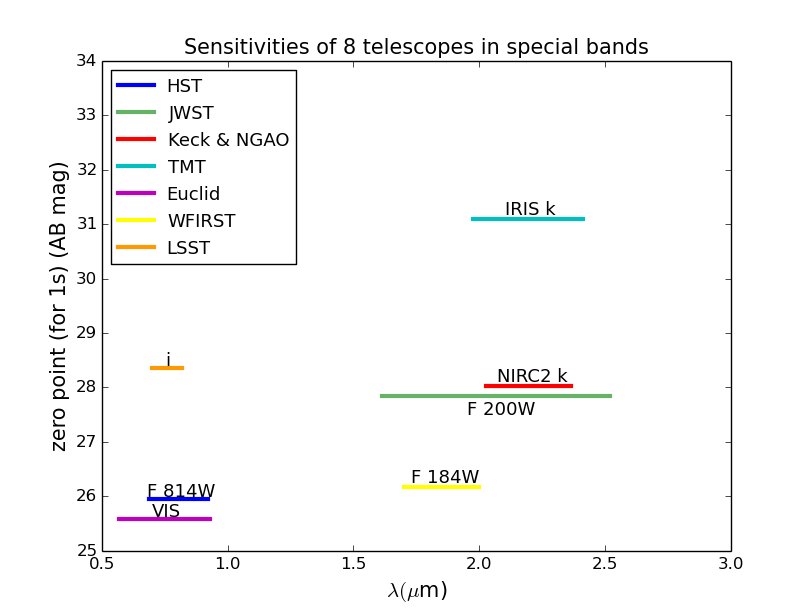
\includegraphics[width=0.9\textwidth]{wavelength_zp.png}
\end{center}
\caption{Zero Points in AB magnitudes of HST (blue), JWST (green), Keck $\&$ NGAO (red), TMT (cyan), Euclid (magenta), WFIRST (yellow) and LSST (orange) in units of per second. Different color bars indicate the wavelength range of each telescope used in this work.}
\label{fig:zp_wavelength}
\end{figure}
% ================================================


% ================================================
\begin{figure}
\begin{center}
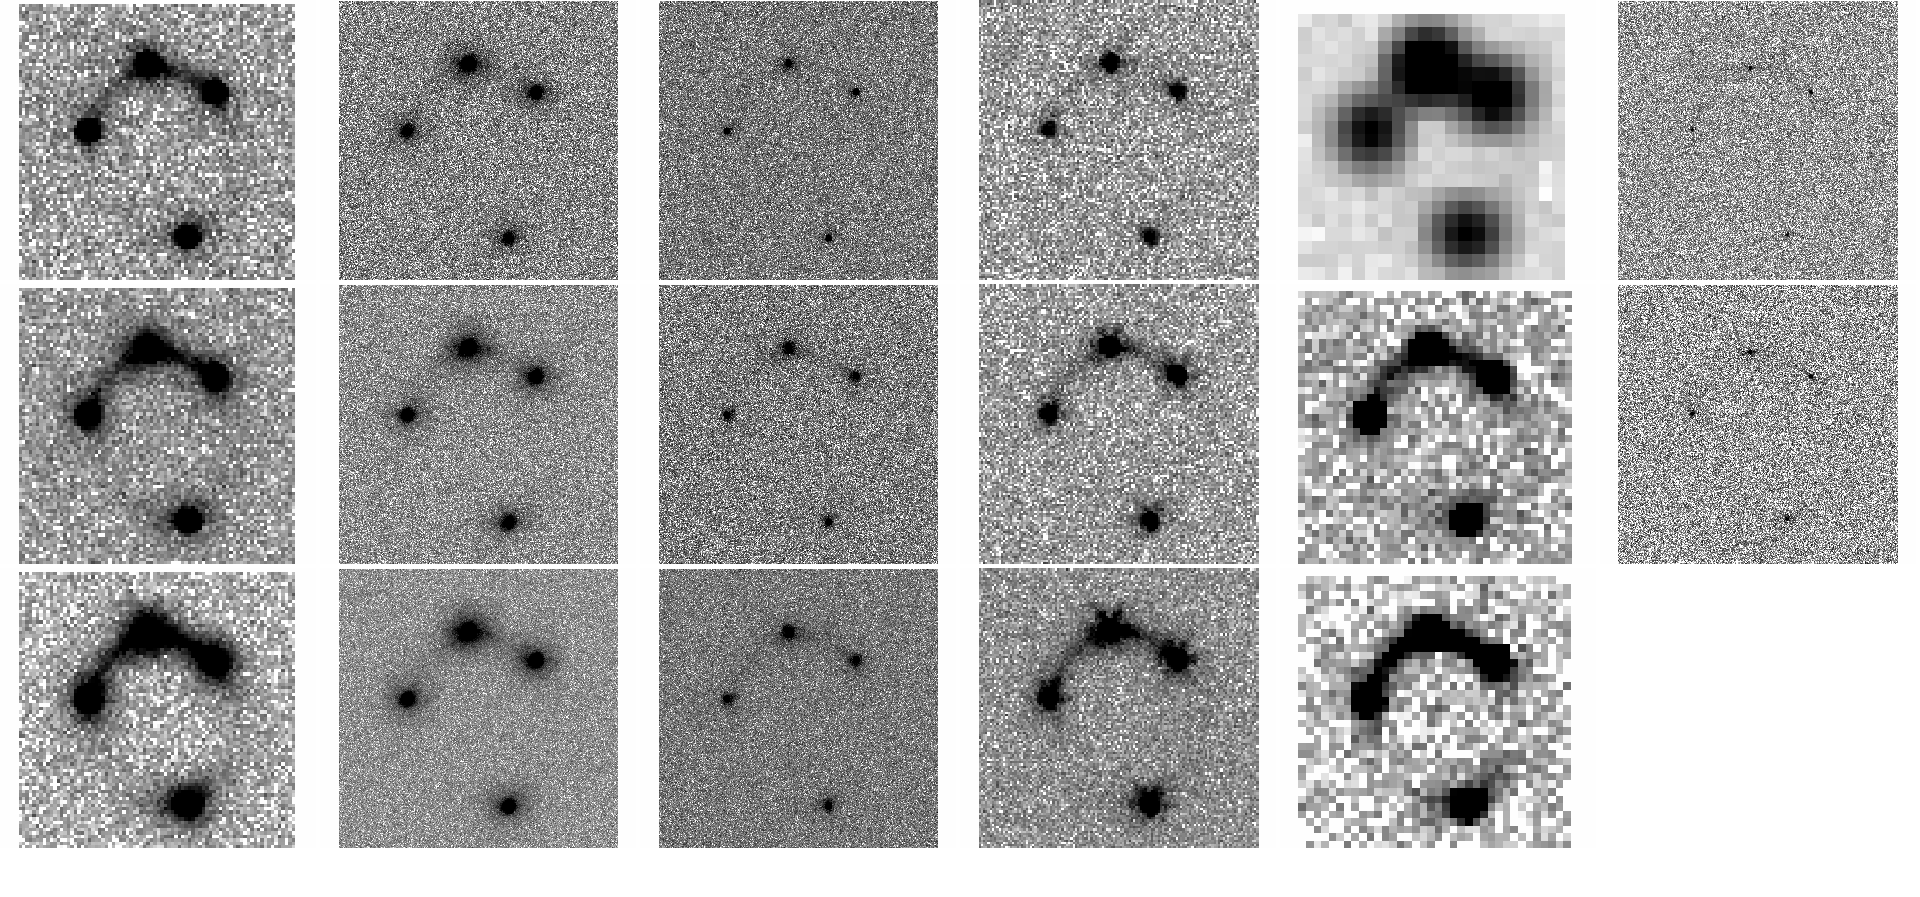
\includegraphics[width=1.0\textwidth]{fainter_system_4QSOimages_all.png}
\end{center}
\caption{Simulated lens system results showing the fainter lens system (4 QSO images in the lens plane). The simulated image pixel scales are all 4$''$ $\times$ 4$''$. The first 4 columns, from left to right, represent HST, Keck, NGAO, and JWST; from top to bottom, correspond to 1/3 $\times$ good exposure time, good exposure time, and 3 $\times$ good exposure time ( See the definition of \textquotedblleft good exposure tine\textquotedblright\ in Section *.*). The fifth column include 3 survey detections by 3 different telescopes, from top to bottom, for LSST, Euclid, and WFIRST respectively. The last column is for TMT with 2 fixed exposure time: 360 seconds and 1080 seconds.}
\label{fig:fainter_4QSOimages_montage}
\end{figure}
% =================================================


% ================================================
\begin{figure}
\begin{center}
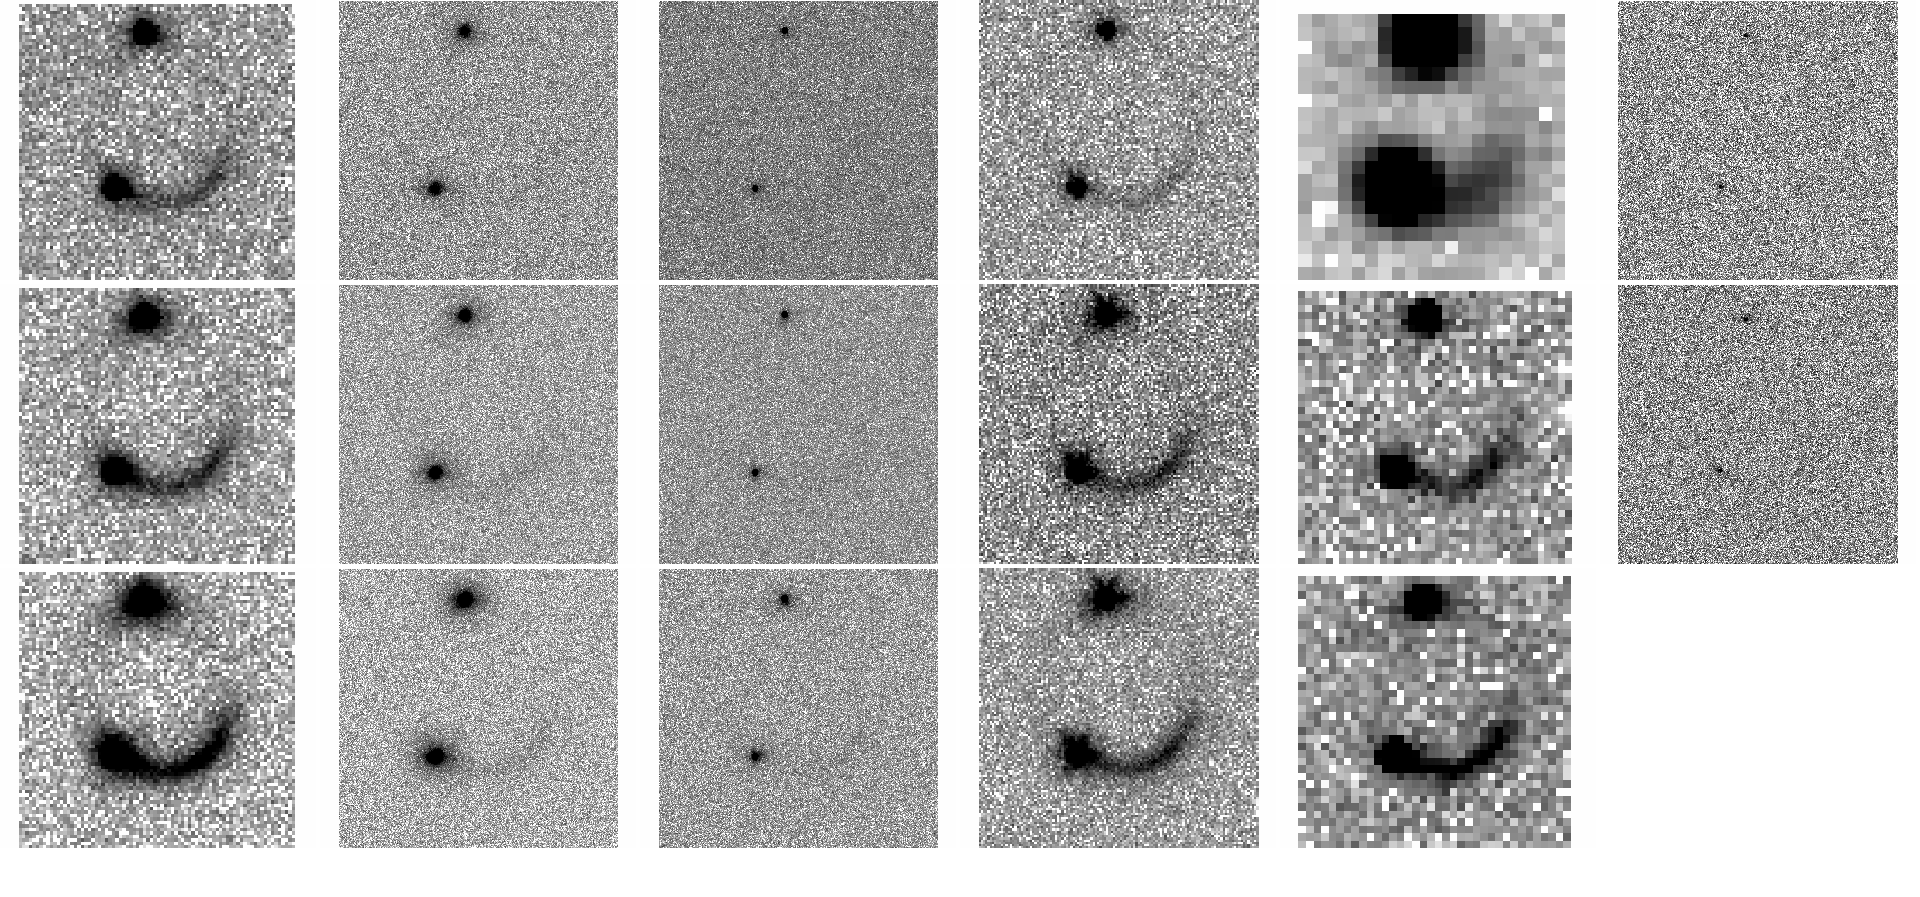
\includegraphics[width=1.0\textwidth]{fainter_system_2QSOimages_all.png}
\end{center}
\caption{Same as Fig. 2, except that the simulated lens system results showing the fainter lens system (2 QSO images in the lens plane).}
\label{fig:fainter_2QSOimages_montage}
\end{figure}
% =================================================


% ================================================
\begin{figure}
\begin{center}
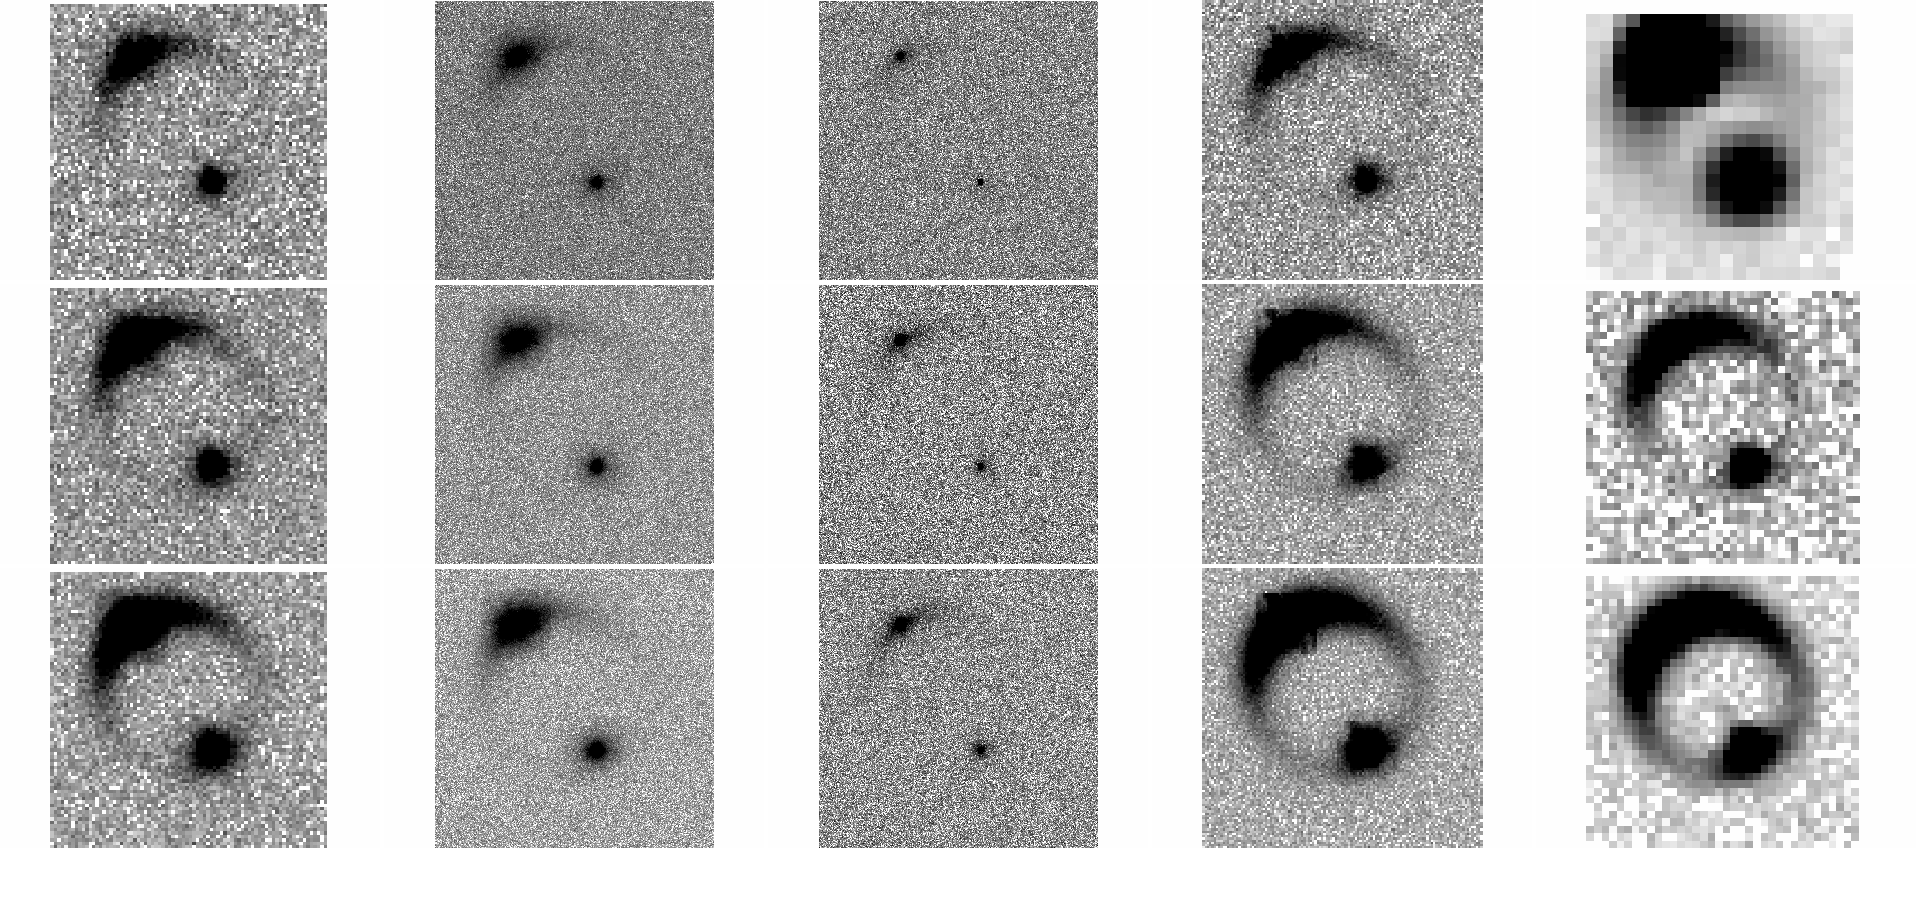
\includegraphics[width=1.0\textwidth]{brighter_system_2QSOimages_all.png}
\end{center}
\caption{Simulated lens system results showing the brighter lens system (2 QSO images in the lens plane). The simulated image pixel scales are all 4$''$ $\times$ 4$''$. The first 3 columns, from left to right, present HST, Keck, and NGAO; from top to bottom, correspond to 1/3 $\times$ good exposure time, good exposure time, and 3 $\times$ good exposure time. The fourth column shows JWST with 3 fixed exposure time: 60 seconds, 180 seconds, and 540 seconds.The last column include 3 survey detections by 3 different telescopes, from top to bottom, for LSST, Euclid, and WFIRST respectively.}
\label{fig:brighter_2QSOimages_montage}
\end{figure}
% =================================================


% ================================================
\begin{figure}
\begin{center}
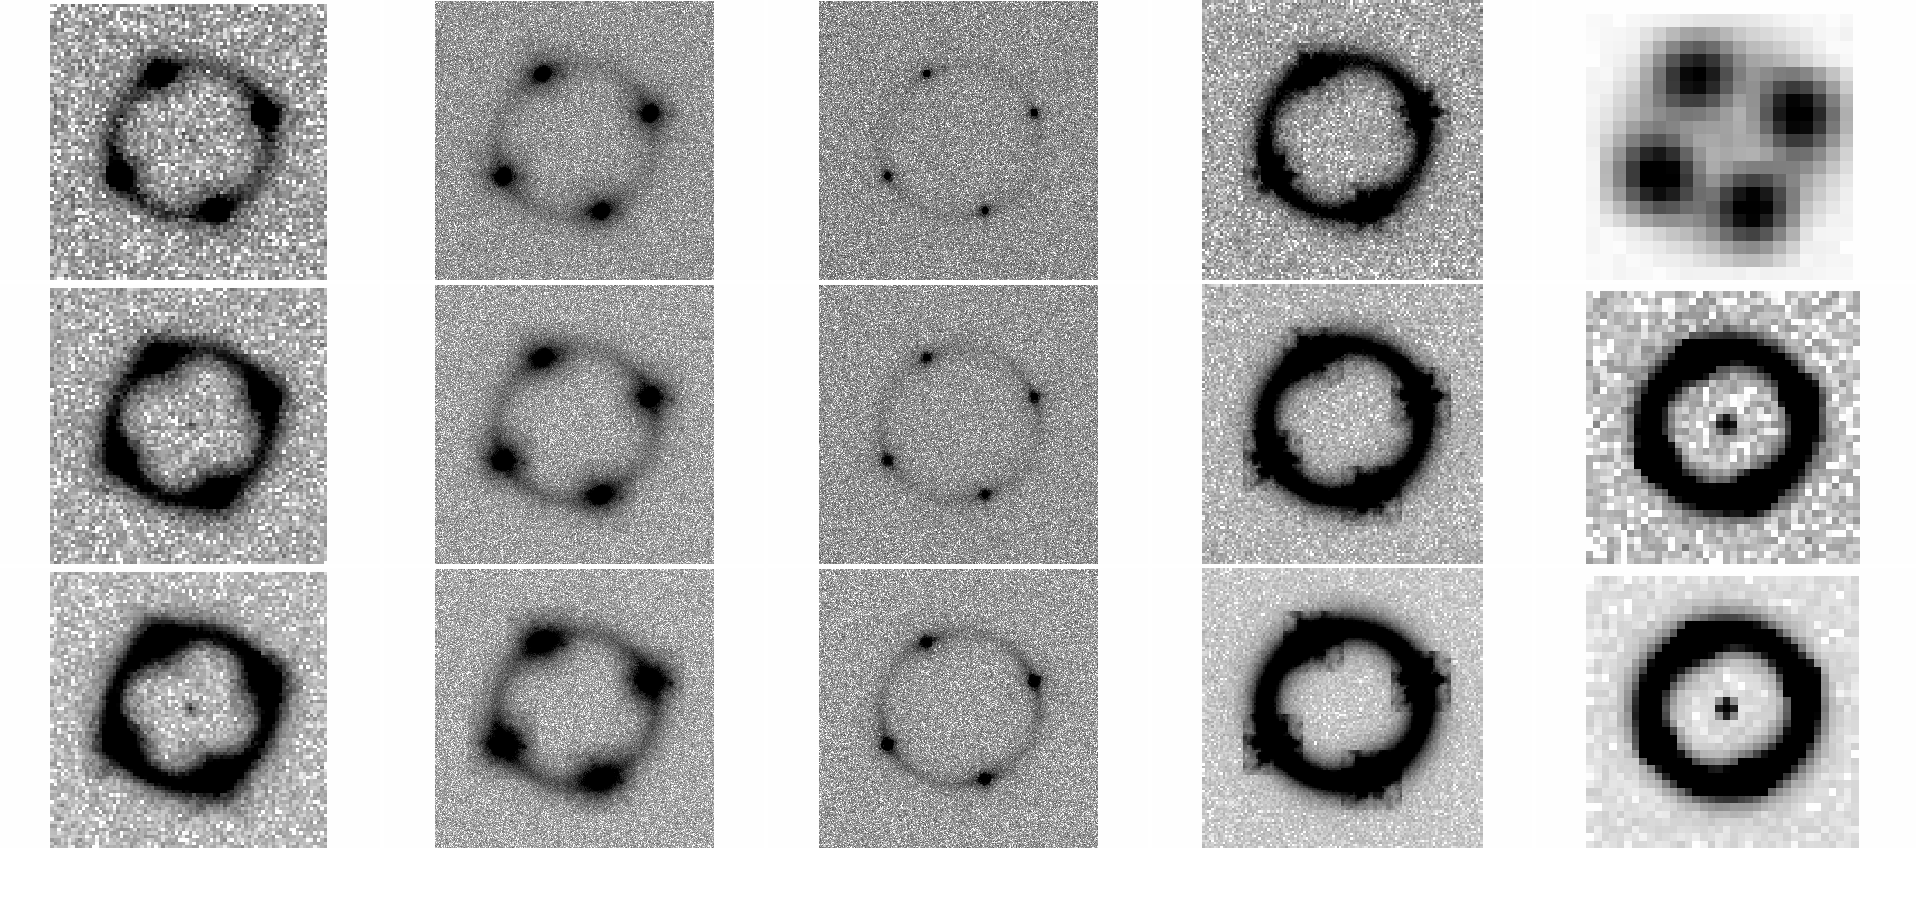
\includegraphics[width=1.0\textwidth]{brighter_system_4QSOimages_all.png}
\end{center}
\caption{Same as Fig. 4, except that the simulated lens system results showing the brighter lens system (4 QSO images in the lens plane). The black spots in the center of the simulated images using HST, Euclid and WFIRST are from the efforts of strong signal pixels, so it's a \textquotedblleft ghost\textquotedblright\ image which can be ignored.}
\label{fig:brighter_4QSOimages_montage}
\end{figure}
% =================================================


% ==================================================
\begin{figure}
\begin{center}
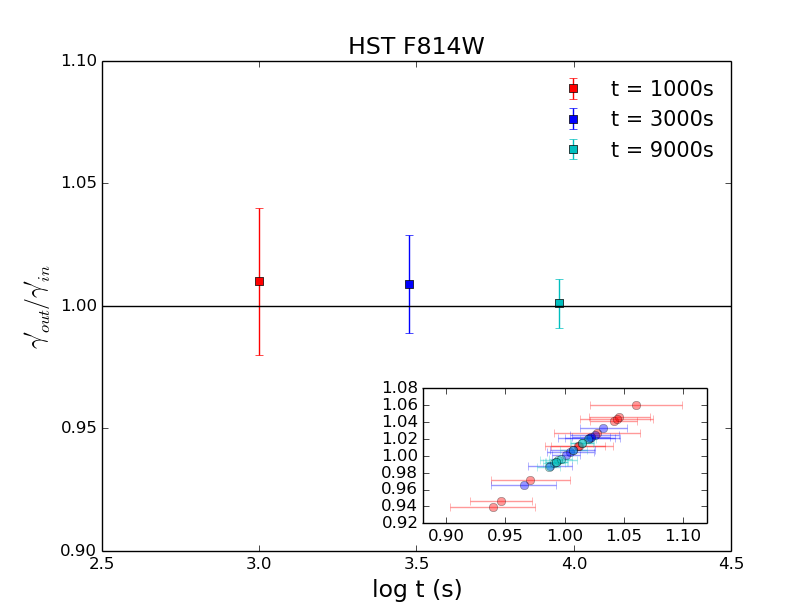
\includegraphics[width=0.48\textwidth]{gamma_135949_4QSOimages_HST.png}
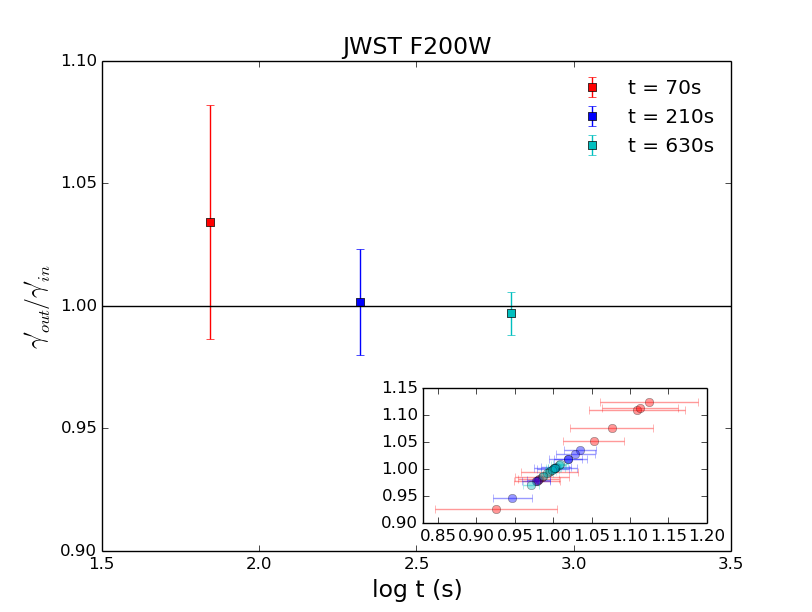
\includegraphics[width=0.48\textwidth]{gamma_135949_4QSOimages_JWST.png} \\
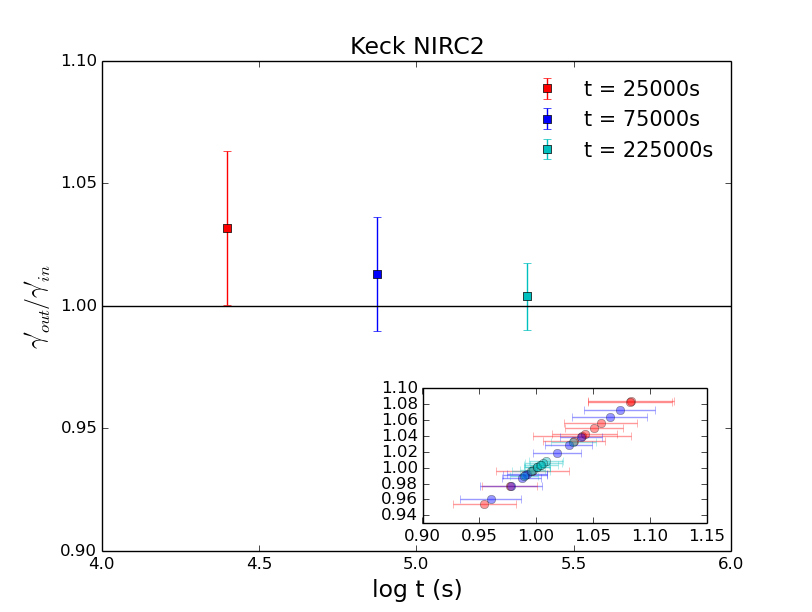
\includegraphics[width=0.48\textwidth]{gamma_135949_4QSOimages_Keck.png}
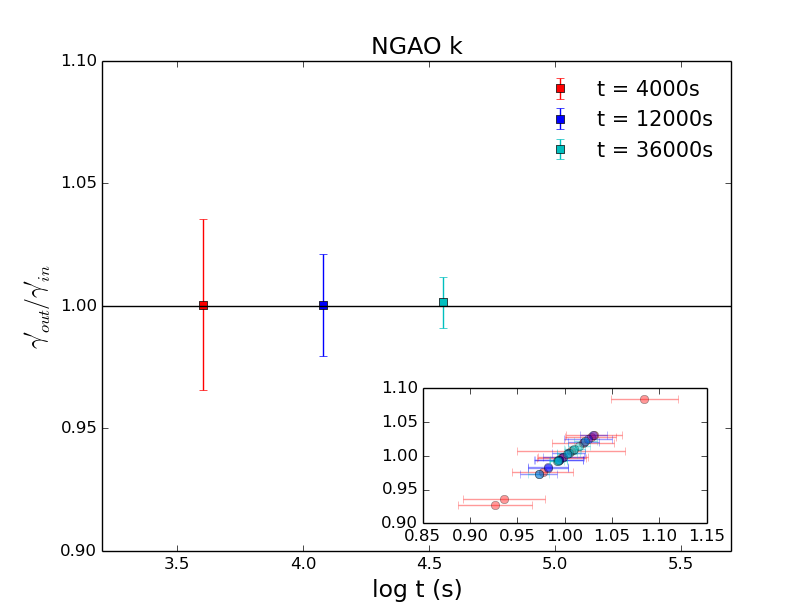
\includegraphics[width=0.48\textwidth]{gamma_135949_4QSOimages_NGAO.png} \\
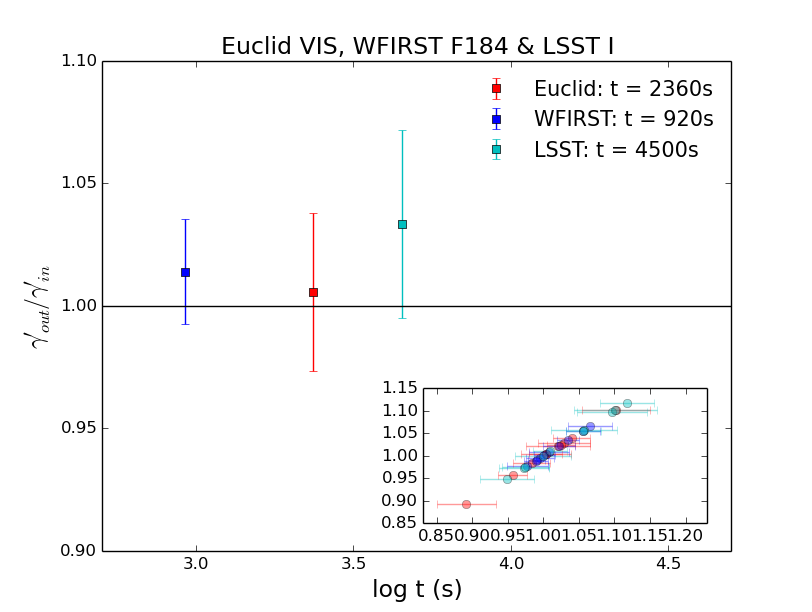
\includegraphics[width=0.48\textwidth]{gamma_135949_4QSOimages_E_W_L.png}
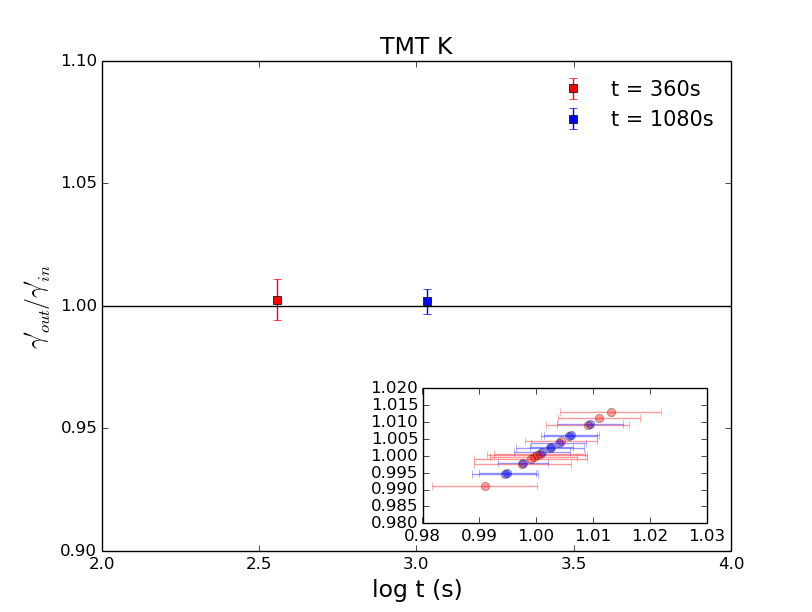
\includegraphics[width=0.48\textwidth]{gamma_135949_4QSOimages_TMT.png}
\end{center}
\caption{The ability of recovering mass slope with respect to different exposure time for a variety of telescopes. This figure shows the fainter lens system with 4 QSO images in the lens plane. $\gamma'_{in}$ is the input SIE mass slope. $\gamma'_{out}$ is drawn from MCMC sampling based on the simulated images given $\gamma'_{in}$. The error bar represents 1$\sigma$ confidence range. The insert in each panel shows all 10 simulation results for each exposure time with the same color coding. Note that both axes represent $\gamma'_{out}/\gamma'_{in}$ whereas error bars are only shown on the x-axis for clarity.}
\label{fig:gamma_fainter_4QSOimages}
\end{figure}
% ======================================================


% ==================================================
\begin{figure}
\begin{center}
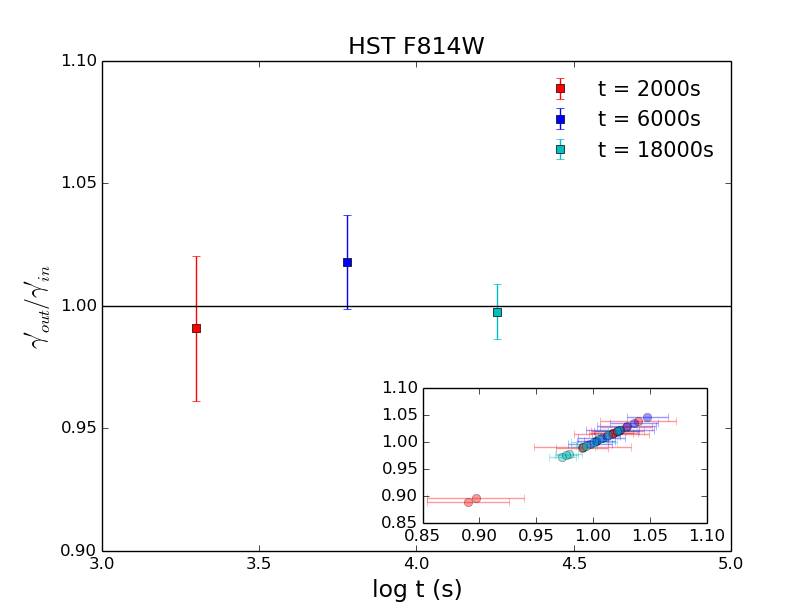
\includegraphics[width=0.48\textwidth]{gamma_135949_anti_2QSOimages_HST.png}
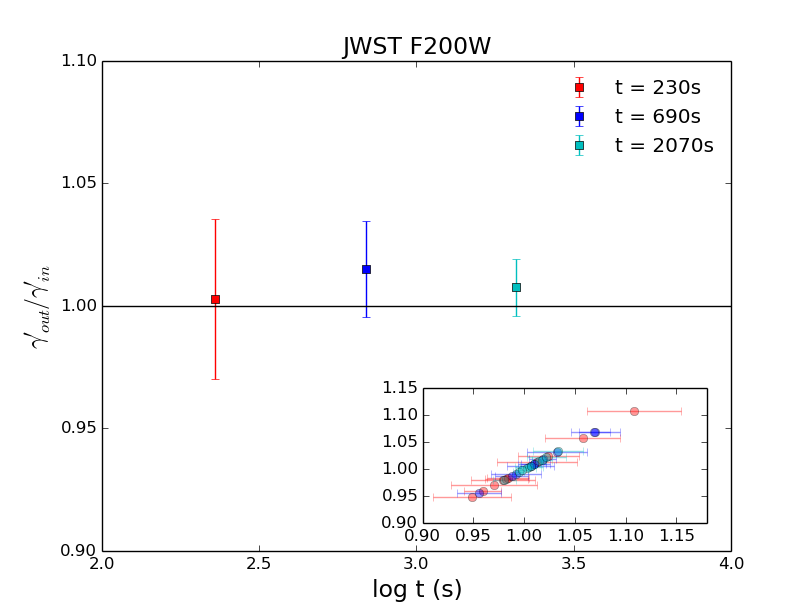
\includegraphics[width=0.48\textwidth]{gamma_135949_anti_2QSOimages_JWST.png} \\
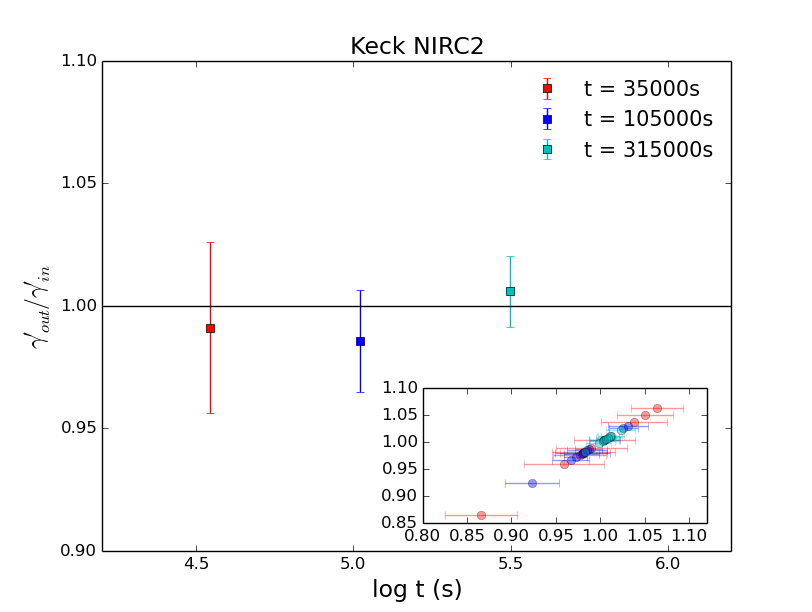
\includegraphics[width=0.48\textwidth]{gamma_135949_anti_2QSOimages_Keck.png}
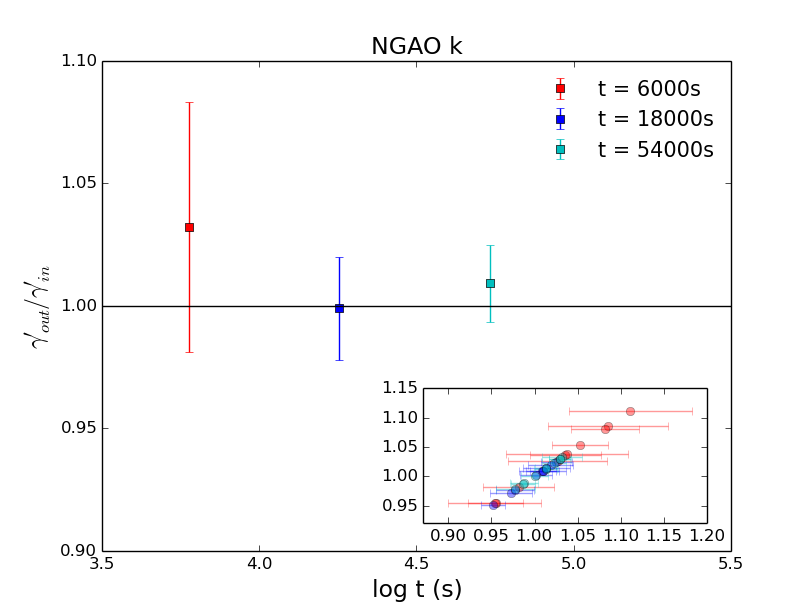
\includegraphics[width=0.48\textwidth]{gamma_135949_anti_2QSOimages_NGAO.png} \\
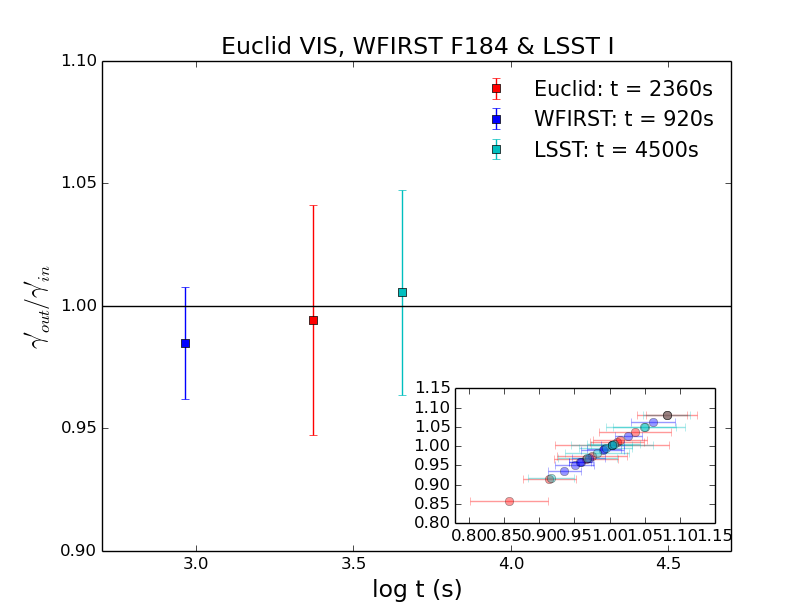
\includegraphics[width=0.48\textwidth]{gamma_135949_anti_2QSOimages_EWL.png}
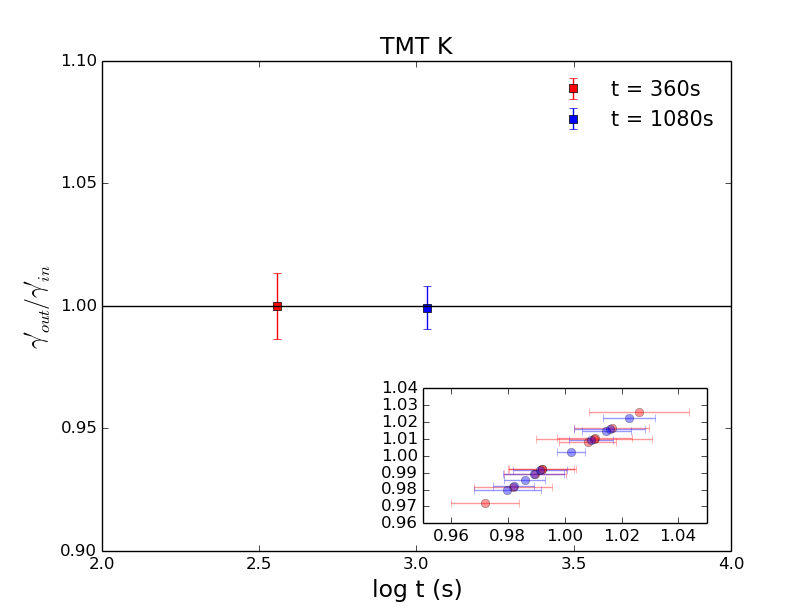
\includegraphics[width=0.48\textwidth]{gamma_135949_anti_2QSOimages_TMT.png}
\end{center}
\caption{Same as Fig. 6, except that this figure is shown for the fainter lens system with 2 QSO images in the lens plane.}
\label{fig:gamma_fainter_2QSOimages}
\end{figure}
% ======================================================


% ==================================================
\begin{figure}
\begin{center}
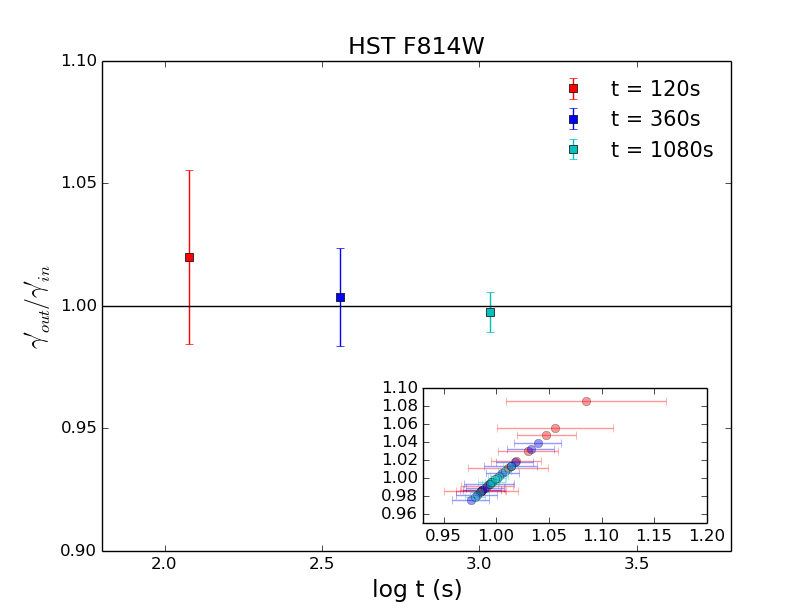
\includegraphics[width=0.48\textwidth]{gamma_0330_2QSOimages_HST.png}
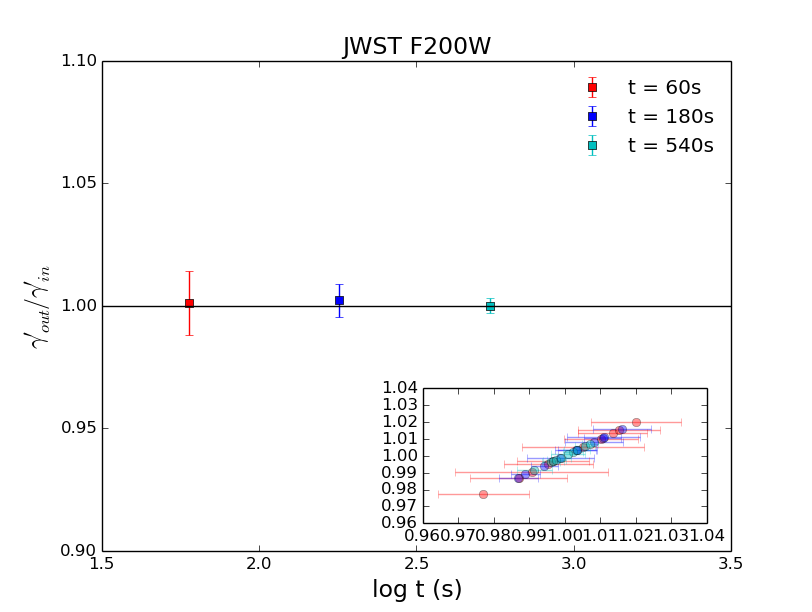
\includegraphics[width=0.48\textwidth]{gamma_0330_2QSOimages_JWST.png} \\
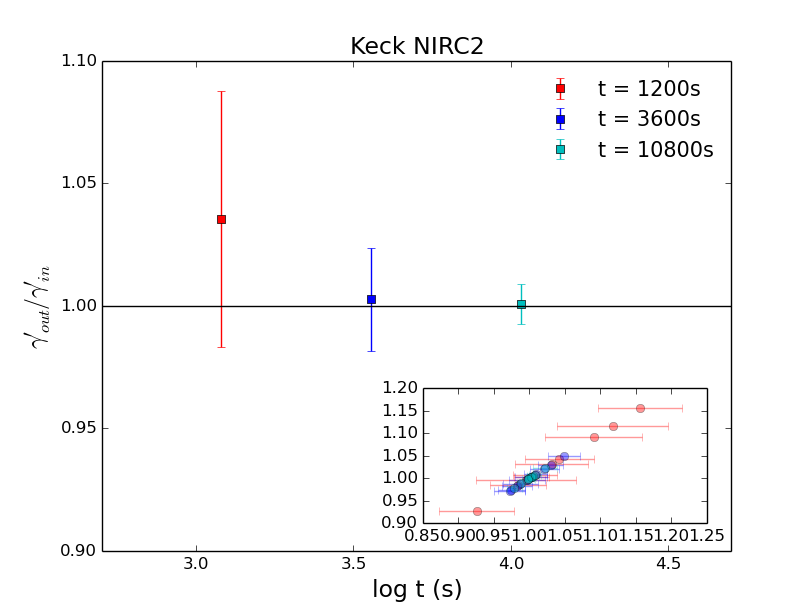
\includegraphics[width=0.48\textwidth]{gamma_0330_2QSOimages_Keck.png}
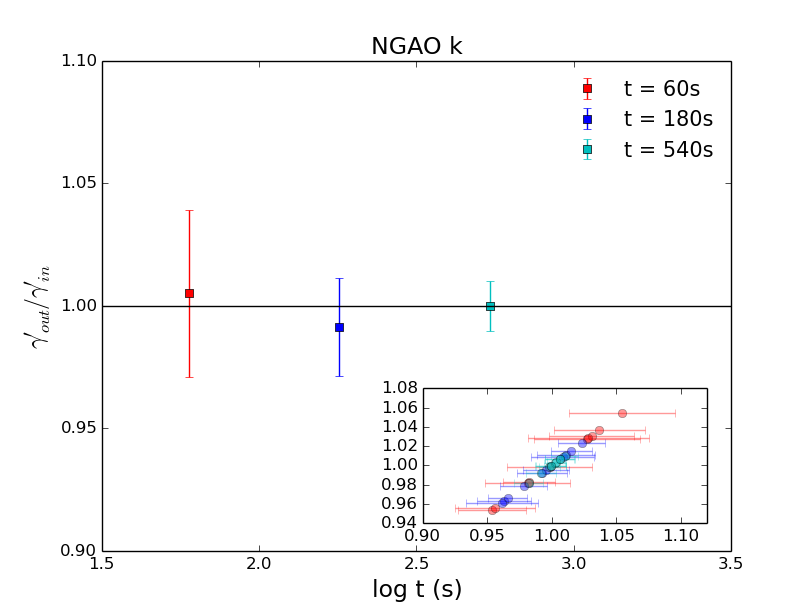
\includegraphics[width=0.48\textwidth]{gamma_0330_2QSOimages_NGAO.png} \\
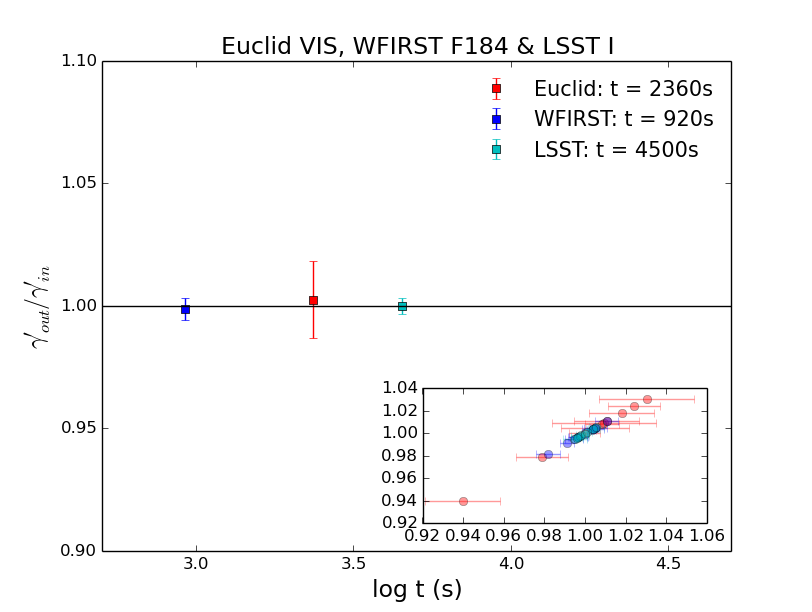
\includegraphics[width=0.48\textwidth]{gamma_0330_2QSOimages_E_W_L.png}
\end{center}
\caption{Same as Fig. 6, except that this figure is shown for the brighter lens system with 2 QSO images in the lens plane.} 
\label{fig:gamma_brighter_2QSOimages}
\end{figure}
% ======================================================


% ==================================================
\begin{figure}
\begin{center}
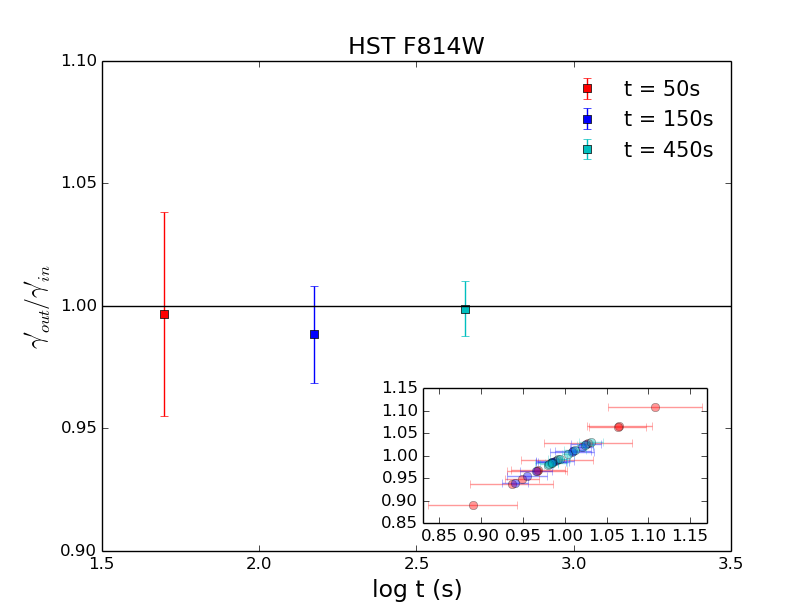
\includegraphics[width=0.48\textwidth]{gamma_0330_anti_4QSOimages_HST.png}
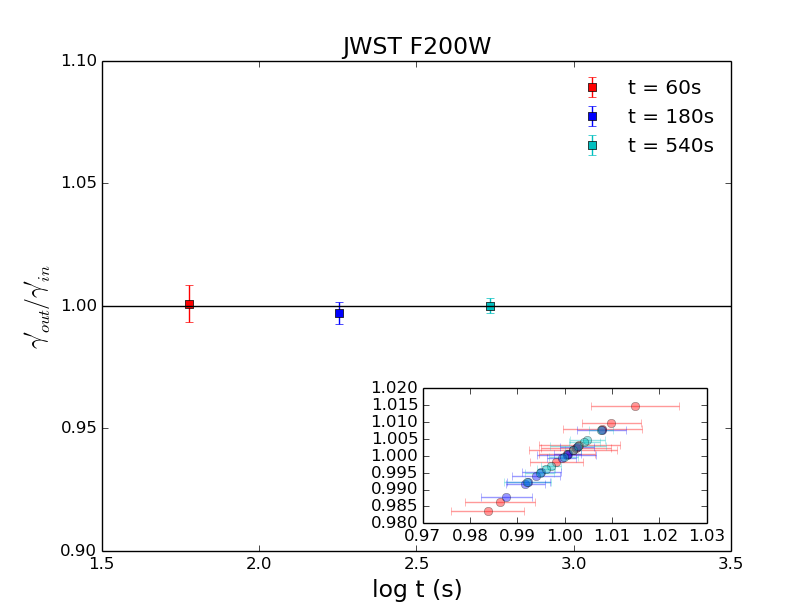
\includegraphics[width=0.48\textwidth]{gamma_0330_anti_4QSOimages_JWST.png} \\
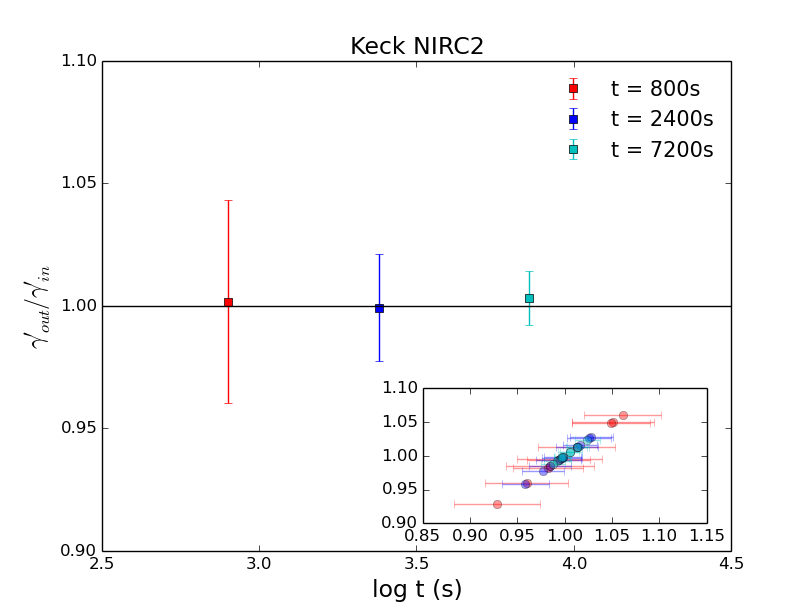
\includegraphics[width=0.48\textwidth]{gamma_0330_anti_4QSOimages_Keck.png}
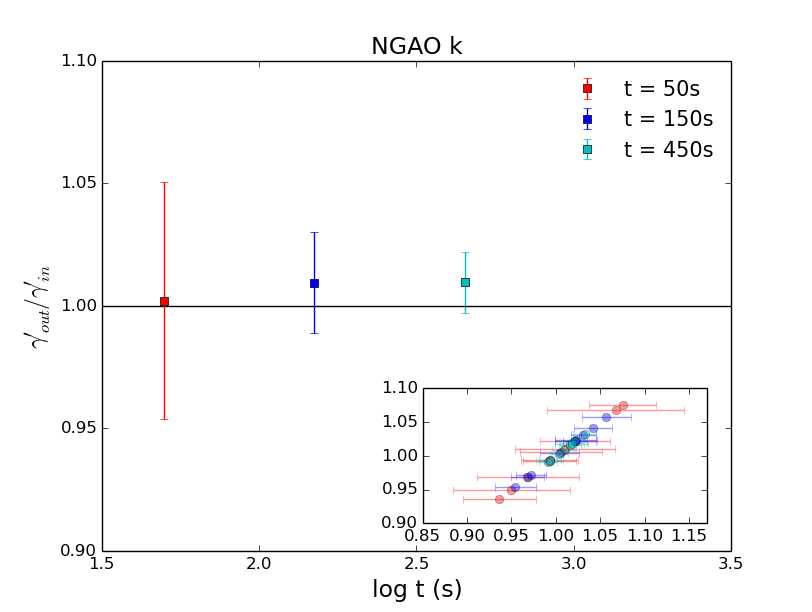
\includegraphics[width=0.48\textwidth]{gamma_0330_anti_4QSOimages_NGAO.png} \\
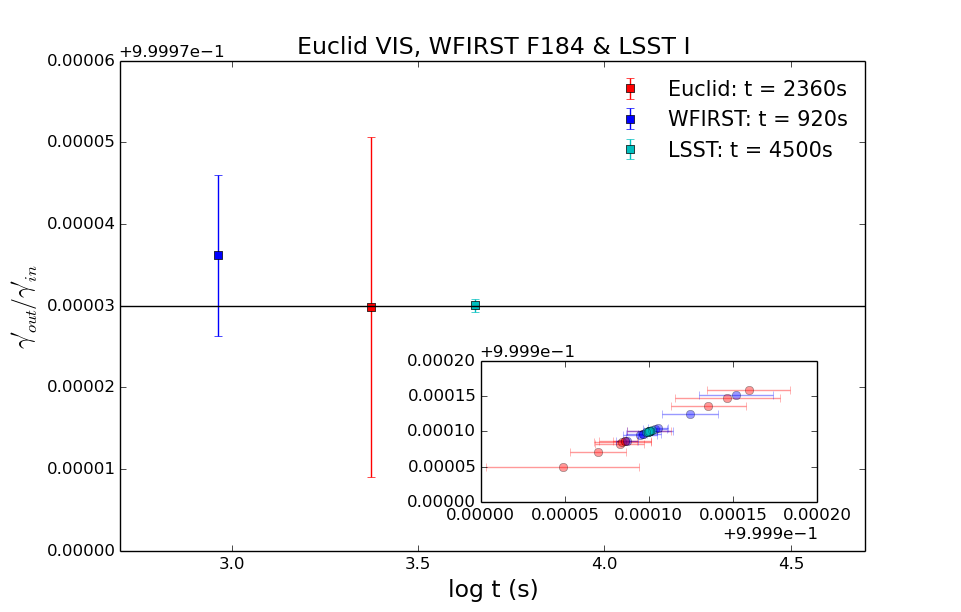
\includegraphics[width=0.48\textwidth]{gamma_0330_anti_4QSOimages_EWL.png}
\end{center}
\caption{Same as Fig. 6, except that this figure is shown for the brighter lens system with 4 QSO images in the lens plane.}
\label{fig:gamma_brighter_4QSOimages}
\end{figure}
% ======================================================

\end{document}